% ---
% Reemplaza líneas 2997–3096 de Docs/Technical_Report.tex.
% Decisiones que lo respaldan: D-005, H-050.
% ---

\subsection{Análisis de la variable objetivo}

\subsubsection{Distribución de clases y balance}

La Figura~\ref{fig:class_distribution} presenta la
distribución de la variable objetivo a nivel global,
por tipo de hallazgo y por split.

\begin{figure}[htbp]
  \centering
  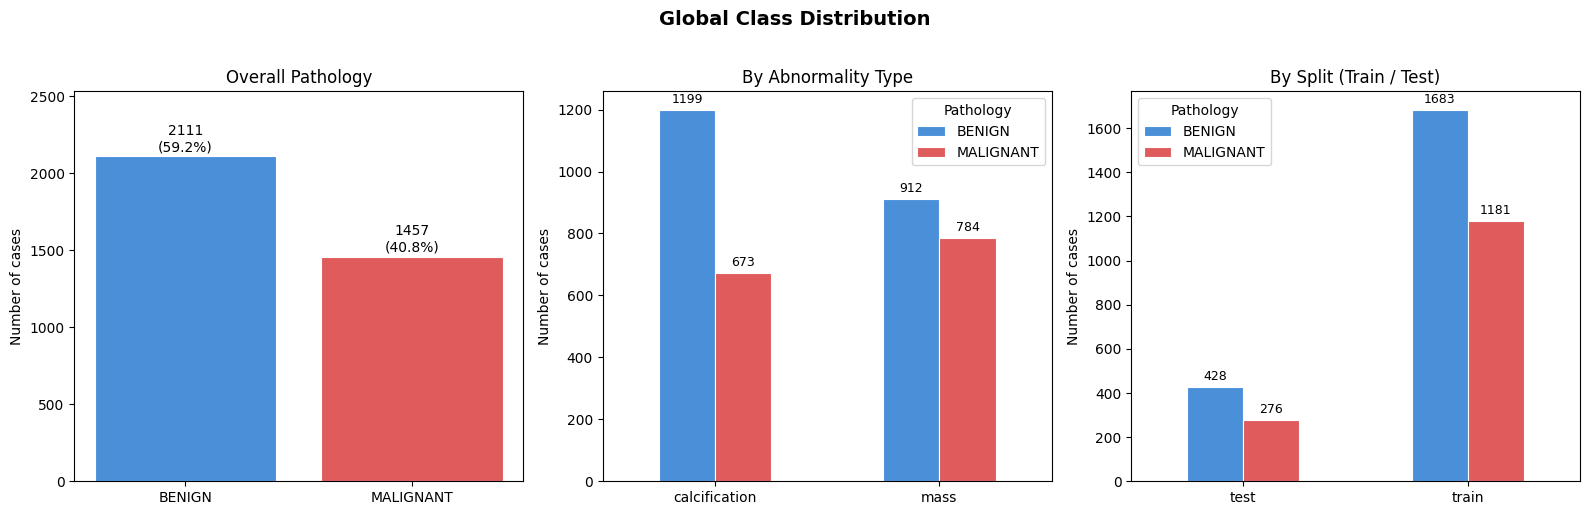
\includegraphics[width=\textwidth]{Figures/B1_class_distribution.png}
  \caption{Distribución de clases global, por tipo de hallazgo y por split train/test.}
  \label{fig:class_distribution}
\end{figure}

% fuente: D-005; 1_EDA.ipynb
El dataset presenta un desbalance global moderado de
1.45:1 (benigno/maligno), que se distribuye de forma
heterogénea entre los dos tipos de hallazgo.
La Figura~\ref{fig:imbalance_by_finding} ilustra
esta asimetría mediante gráficas de pastel por
subconjunto.

\begin{figure}[htbp]
  \centering
  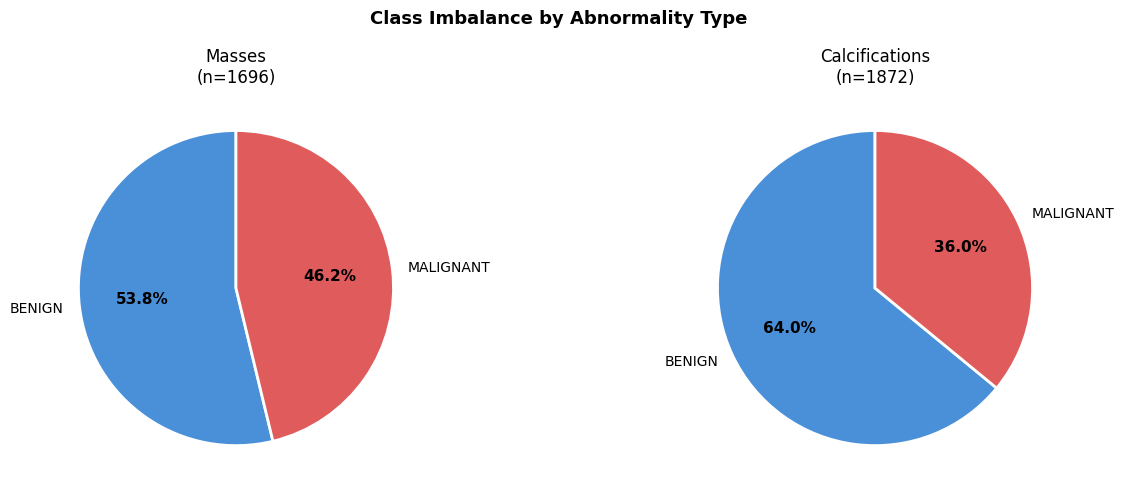
\includegraphics[width=0.75\textwidth]{Figures/B2_imbalance_by_finding.png}
  \caption{Desbalance de clases por tipo de hallazgo.}
  \label{fig:imbalance_by_finding}
\end{figure}

% fuente: D-005; 1_EDA.ipynb
Las masas presentan un balance casi simétrico (ratio
1.16:1), con 912 casos benignos y 784 malignos.
Las calcificaciones muestran un desbalance más
pronunciado (ratio 1.78:1), con 1\,199 casos benignos
frente a 673 malignos. Esta asimetría tiene una
implicación metodológica directa: se requiere
ponderación de clases (\texttt{class\_weight=balanced})
durante el entrenamiento del MLP, aplicada de forma
independiente para cada subconjunto, como se
especifica en el requerimiento RF-19.

\subsubsection{Distribución BI-RADS}

La Figura~\ref{fig:birads_distribution} muestra la
distribución de la categoría BI-RADS por patología
y tipo de hallazgo.

\begin{figure}[htbp]
  \centering
  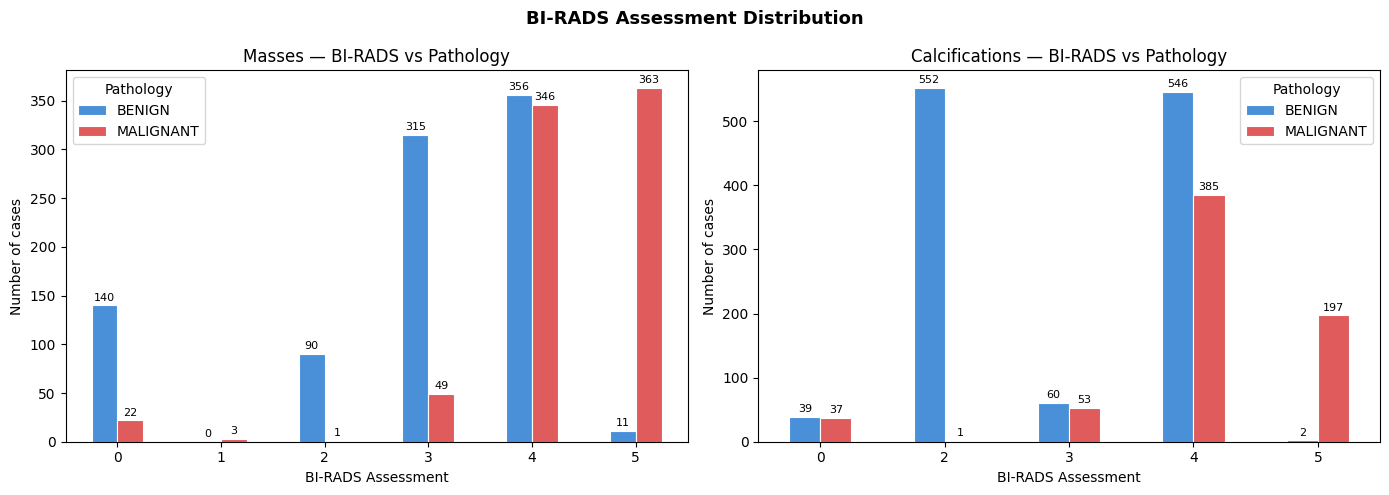
\includegraphics[width=\textwidth]{Figures/B3_birads_distribution.png}
  \caption{Distribución de categorías BI-RADS por patología y tipo de hallazgo.}
  \label{fig:birads_distribution}
\end{figure}

% fuente: D-005; 1_EDA.ipynb
Se observa una concentración de casos malignos en las
categorías BI-RADS 4 y 5 (sospechoso y altamente
sospechoso), mientras que los casos benignos se
distribuyen predominantemente en las categorías 2 y
3. Esta distribución valida la coherencia clínica del
dataset: la categoría BI-RADS refleja directamente
el nivel de sospecha de malignidad asignado por el
radiólogo.

\subsubsection{Análisis de subtlety}

% fuente: D-005; 1_EDA.ipynb
\begin{figure}[htbp]
  \centering
  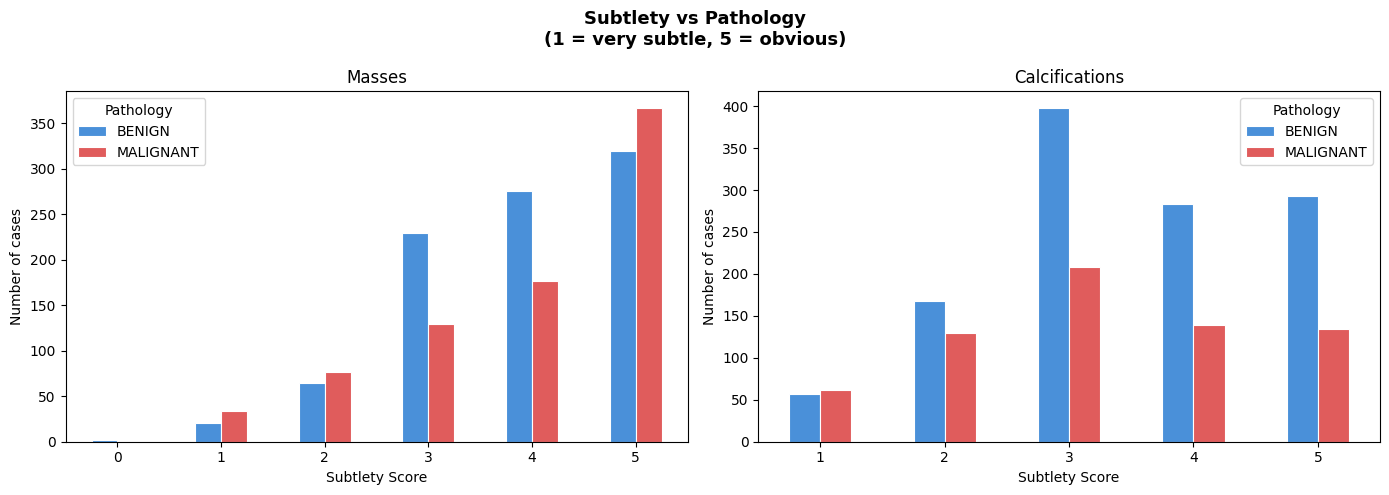
\includegraphics[width=\textwidth]{Figures/B4_subtlety_distribution.png}
  \caption{Distribución de \textit{subtlety} por patología y tipo de hallazgo (1\,=\,muy sutil, 5\,=\,obvio).}
  \label{fig:subtlety_distribution}
\end{figure}

% fuente: D-005; 1_EDA.ipynb
La media de \textit{subtlety} en casos malignos
(3.1 para masas, 2.8 para calcificaciones) es
ligeramente inferior a la de casos benignos (3.4 y
3.2 respectivamente), aunque la diferencia es pequeña.
Este hallazgo refuta la intuición de que las lesiones
malignas son necesariamente más difíciles de detectar
visualmente: la dificultad de detección es
aproximadamente ortogonal a la patología, lo que
explica parcialmente por qué los modelos de deep
learning enfrentan dificultades de generalización al
no poder apoyarse en la obviedad visual como señal
discriminativa.
